%----------------------------------------------------------------------------------------
%    Lecture 2: From RBC to IS–LM (template-compatible, uses your v2 preamble)
%----------------------------------------------------------------------------------------

\documentclass[aspectratio=169,xcolor=dvipsnames]{beamer}
\usetheme{SimpleDarkBlue}

\usepackage{hyperref}
\usepackage{graphicx}
\usepackage{booktabs}
\usepackage{appendixnumberbeamer}
\usepackage{amsmath}
\usepackage{booktabs}
\usepackage{xcolor} % For custom colors
\usepackage{tikz} % For styling enumerate numbers
\usepackage{tcolorbox} % For colored box styling
\usepackage{amsmath, amsfonts, amssymb, amsthm} % Math related
\usepackage{natbib}
\usepackage{iftex}
\usepackage{pgfpages} % beamer speaker notes

% --- Speaker notes (default: hidden). ---
% Uncomment ONE of the following lines when you want presenter notes in the PDF.
% \setbeameroption{show notes}
\setbeameroption{show notes on second screen=right}
% \setbeameroption{hide notes}

% --- Font handling: compile with pdfLaTeX here; switch to LuaLaTeX locally if desired ---
\ifPDFTeX
  \usepackage[T1]{fontenc}
  \usepackage{lmodern}
  \usepackage{microtype}
\else
  \usepackage{fontspec}
  \usepackage{luatexja}
  \setmainfont{Alegreya Sans Light}[
    ItalicFont={* Italic},
    BoldFont={Alegreya Sans Medium},
    BoldItalicFont={Alegreya Sans Medium Italic}]
  \setsansfont{Alegreya Sans Light}[
    ItalicFont={* Italic},
    BoldFont={Alegreya Sans Medium},
    BoldItalicFont={Alegreya Sans Medium Italic}]
\fi

% ---------------- %
% color definition %
% ---------------- %
\definecolor{main}{HTML}{23373B}
\definecolor{pink}{RGB}{180, 50, 110}
\definecolor{orange}{HTML}{FF8000}
\definecolor{red}{HTML}{990000}
\definecolor{blue}{HTML}{004C99}
\definecolor{lightgray}{HTML}{E7E7E7}
\definecolor{gray}{RGB}{90, 90, 90}

% ------------ %
% beamerbutton %
% ------------ %
\newcommand{\goto}[2]{\hyperlink{#2}{\beamergotobutton{#1}}}
\newcommand{\return}[2]{\hyperlink{#2}{\beamerreturnbutton{#1}}}
\newcommand{\extgoto}[2]{\href{#2}{\beamergotobutton{#1}}}

% ------------------------------------ %
% Section title page with Huge bf text %
% ------------------------------------ %
\AtBeginSection[]{
  \begin{frame}[noframenumbering, plain]
    \Huge{\centerline{\textbf{\insertsection}}}
  \end{frame}
}

\usepackage[mode=tex]{standalone}
\usepackage{tikz}
\usetikzlibrary{decorations}
\usetikzlibrary{decorations.pathreplacing, intersections}
\usepackage{pgfplots}
\usetikzlibrary{calc,positioning}
\usepgfplotslibrary{fillbetween}
\pgfplotsset{compat=newest, scale only axis, width = 10cm}

%%% automatically add spaces into enumerate and itemize environment
\let\tempone\itemize
\let\temptwo\enditemize
\renewenvironment{itemize}{\tempone\addtolength{\itemsep}{\fill}}{\temptwo}
\let\tempa\enumerate
\let\tempb\endenumerate
\renewenvironment{enumerate}{\tempa\addtolength{\itemsep}{\fill}}{\tempb}

%%=============================================================
%%  FOOTLINE TEMPLATE
%%=============================================================
\defbeamertemplate*{footline}{shadow theme}{%
    \leavevmode\hbox{%
        \hypersetup{linkcolor=white,urlcolor=white,citecolor=white}
        \begin{beamercolorbox}[wd=1.02\paperwidth, ht=2.5ex, dp=1.125ex, leftskip=.3cm plus1fil, rightskip=0.3cm]{author in head/foot}%
            \insertsectionnavigationhorizontal{.80\textwidth}{}{} \hspace{.3cm} \hfill \#\ \insertframenumber \ / \ \inserttotalframenumber%
        \end{beamercolorbox}%
    }%
}
\setbeamertemplate{footline}[shadow theme]

%----------------------------------------------------------------------------------------
%    TITLE PAGE
%----------------------------------------------------------------------------------------

\title[Lecture 2: IS--LM]{Intermediate Macroeconomics II\\\vspace{4pt}Lecture 2: From RBC to IS--LM}
\author[Hui-Jun Chen]{Hui-Jun Chen}
\institute[]{National Tsing Hua University}
\date{Spring 2026}

% Put your jpg files in one of these folders (or edit as needed)
\graphicspath{{figures/}{figs/}{./}}

%----------------------------------------------------------------------------------------
%    PRESENTATION SLIDES
%----------------------------------------------------------------------------------------

\begin{document}

%------------------------------------------------
\begin{frame}[plain,noframenumbering]
    \titlepage
\end{frame}

%------------------------------------------------
\begin{frame}{Today: why we move from RBC to IS--LM}
\small
\begin{itemize}
\item Last time (RBC): output and the \textbf{real interest rate} are pinned down by \textbf{real} constraints and intertemporal choices.
\item This semester's focus: \textbf{inflation and the price level} --- so we must add a \textbf{nominal side}.
\item IS--LM is our \textbf{first bridge model}:
\begin{itemize}
\item IS = goods market equilibrium (a reduced-form view of intertemporal demand)
\item LM = money market equilibrium (how nominal variables enter)
\end{itemize}
\end{itemize}

\begin{block}{What you should be able to do after Lecture 2}
Explain how \textbf{goods demand} and \textbf{money demand} jointly determine $(Y,r)$ in the short run, and how policy shifts the system.
\end{block}
\note{\small
\textbf{Opening (1--2 min).} Remind students what last lecture delivered: a real allocation + a real rate.\\
\textbf{Motivation.} This semester is about $P$ and $\pi$: we need nominal variables on the board.\\
\textbf{Learning goals.} Tell them: today is all about reading comparative statics from diagrams.\\
\textbf{Quick check.} Ask: ``In RBC, what pins down the real interest rate?'' (preferences/technology).\\
\textbf{Transition.} ``IS--LM is not the final model---it is our first bridge to inflation.''
}
\end{frame}

%------------------------------------------------
\section{Recap: what RBC gives us}

%------------------------------------------------
\begin{frame}{RBC in one slide: what we learned (and what we did \emph{not})}
\small
\begin{itemize}
\item \textbf{RBC core idea:} flexible prices $\Rightarrow$ markets clear $\Rightarrow$ output is tied to productivity and factor supply.
\item The key intertemporal price is the \textbf{real rate} $r_t$:
\[
1 = \beta \,\mathbb{E}_t\left[\frac{u'(C_{t+1})}{u'(C_t)}(1+r_t)\right].
\]
\item In that world, monetary variables are typically \textbf{neutral} for real allocations (classical dichotomy logic).
\end{itemize}

\begin{block}{So why add IS--LM?}
Because once we care about \textbf{nominal interest rates, money demand, and the price level}, we need equations that speak to them explicitly.
\end{block}
\note{\small
\textbf{Emphasize dichotomy.} RBC delivers $Y$ and $r$ from real forces; nominal side is absent/irrelevant for allocations.\\
\textbf{Key phrase.} ``RBC is silent about the \emph{price level} unless we add a nominal anchor.''\\
\textbf{Bridge idea.} IS--LM adds a money market and a nominal rate so we can start asking: what happens to $Y$ and $P$ when policy moves?\\
\textbf{Pitfall to avoid.} Students may think ``money doesn't matter'' always---clarify: that is a property of the flexible-price benchmark.
}
\end{frame}

\begin{frame}{Competitive Equilibrium}
\label{slide:Competitive_Equilibrium}
    \begin{center}
        \scriptsize Figure 11.21  The Complete Real Intertemporal Model
    \end{center}
    \begin{columns}
        \begin{column}{0.5\textwidth}
            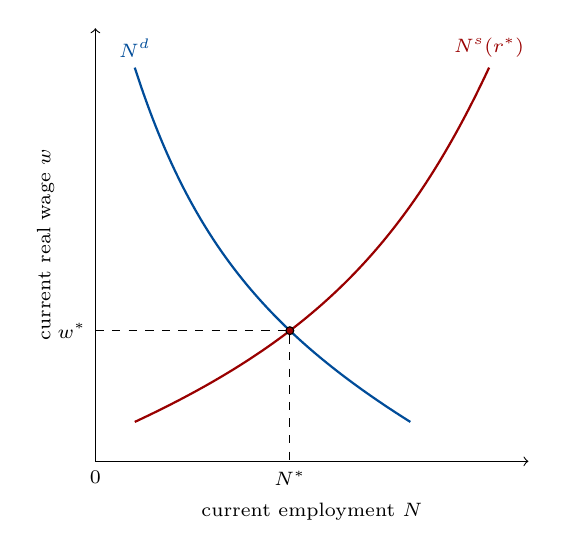
\begin{tikzpicture}[domain=0:5]
                \tikzstyle{every node}=[font=\scriptsize]
                \pgfmathsetmacro{\x}{5};
                \pgfmathsetmacro{\y}{5};
                % \draw[very thin,color=gray, step=0.1] (0,0) grid (\x, \y); % gray grid
                \draw[->] (0,0) node[below]{ $ 0 $  } -- node[below, yshift = -0.4cm]{current employment $ N $} (\x + 0.5,0) ;   % label x axis
                \draw[->] (0,0) -- node[above, rotate=90, yshift = 0.4cm]{current real wage $w$} (0,\y + 0.5) ;   % label y axis
                \draw[thick, red, name path = aa]
                    (\x, \y)
                    node[above]{$N^{s}( r^{*} )$}
                    to[bend left=20]
                    (0.5, 0.5);
                \draw[thick, blue, name path = bb]
                    (0.5, \y)
                    node[above]{$N^{d}$}
                    to[bend right=20]
                    (4, 0.5);
                \path[name intersections={of=aa and bb, by=b}];
                \node[draw,fill=red,circle,inner sep=1pt] at (b) {};
                \path (b); \pgfgetlastxy{\xcoord}{\ycoord};
                \coordinate (b_x) at (\xcoord, 0);
                \coordinate (b_y) at (0, \ycoord);
                \draw[dashed] (b_y) node[left]{$w^{*}$}  -- (b) -- (b_x) node[below]{$N^{*}$};

            \end{tikzpicture}
        \end{column}
        \begin{column}{0.5\textwidth}

            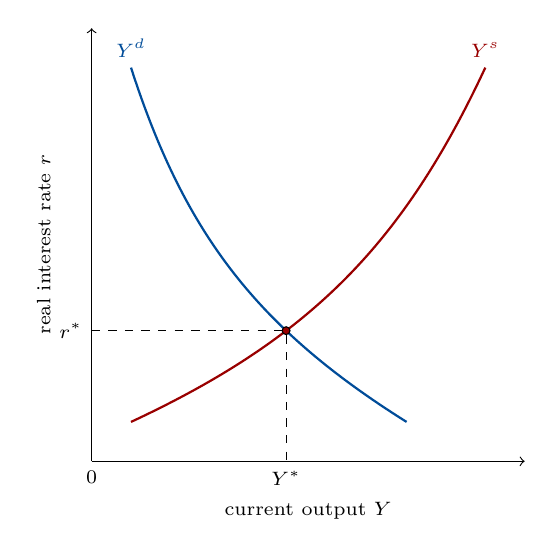
\begin{tikzpicture}[domain=0:5]
                \tikzstyle{every node}=[font=\scriptsize]
                \pgfmathsetmacro{\x}{5};
                \pgfmathsetmacro{\y}{5};
                % \draw[very thin,color=gray, step=0.1] (0,0) grid (\x, \y); % gray grid
                \draw[->] (0,0) node[below]{ $ 0 $  } -- node[below, yshift = -0.4cm]{current output $ Y $} (\x + 0.5,0) ;   % label x axis
                \draw[->] (0,0) -- node[above, rotate=90, yshift = 0.4cm]{real interest rate $r$} (0,\y + 0.5) ;   % label y axis
                \draw[thick, red, name path = aa]
                    (\x, \y)
                    node[above]{$Y^{s}$}
                    to[bend left=20]
                    (0.5, 0.5);
                \draw[thick, blue, name path = bb]
                    (0.5, \y)
                    node[above]{$Y^{d}$}
                    to[bend right=20]
                    (4, 0.5);
                \path[name intersections={of=aa and bb, by=a}];
                \node[draw,fill=red,circle,inner sep=1pt] at (a) {};
                \path (a); \pgfgetlastxy{\xcoord}{\ycoord};
                \coordinate (a_x) at (\xcoord, 0);
                \coordinate (a_y) at (0, \ycoord);
                \draw[dashed] (a_y) node[left]{$r^{*}$}  -- (a) -- (a_x) node[below]{$Y^{*}$};

            \end{tikzpicture}
        \end{column}
    \end{columns}
\note{\small
\textbf{Purpose.} This is your ``baseline map'': with flexible prices, two real markets pin down $(N,w)$ and $(Y,r)$.\\
\textbf{Walk-through.} Left panel: $N^d$ and $N^s(r^*)$ intersect at $(N^*,w^*)$. Right panel: goods market $Y^d$ and $Y^s$ intersect at $(Y^*,r^*)$.\\
\textbf{Key contrast.} In RBC, $r$ moves because of real forces; money is not in the picture.\\
\textbf{Transition line.} ``Now we add a \\emph{third} market: money. That extra condition will change how we think about interest rates in the short run.''
}
\end{frame}

%------------------------------------------------
\begin{frame}{A clean map: same economy, more markets on the board}
\small
Think of the macro economy as \textbf{two big clearing conditions} plus a policy rule:

\begin{itemize}
\item \textbf{Goods market:} planned spending equals production (IS logic).
\item \textbf{Money market:} money supplied equals money demanded (LM logic).
\item \textbf{Policy:} central bank and fiscal authority pick instruments / regimes.
\end{itemize}

\begin{block}{Important perspective}
IS--LM is a \textbf{different representation} that highlights \textbf{demand} and \textbf{nominal variables}. Later we replace its weak spots with NK microfoundations.
\end{block}
\note{\small
\textbf{Big picture.} Tell students: every macro model is ``markets + policy.'' IS--LM just chooses a different pair of markets to foreground.\\
\textbf{Board plan.} Draw two boxes on the board: (1) Goods market clearing (IS), (2) Money market clearing (LM). Add a third box called ``Policy regime.''\\
\textbf{Expectation management.} Acknowledge limitations up front: IS--LM is intuition/benchmark; NK will microfound the same logic with expectations and price setting.
}
\end{frame}

%------------------------------------------------
\section{Money market and LM}

%------------------------------------------------
\begin{frame}{Step 1: Money demand (why people hold money)}
\small
\begin{columns}
\begin{column}{0.62\textwidth}
\centering
\includegraphics[width=\linewidth]{moneyd.jpg}
\end{column}
\begin{column}{0.38\textwidth}
\begin{itemize}
\item Money provides \textbf{liquidity} (transactions/convenience).
\item Holding money has an \textbf{opportunity cost}: the interest you could earn on bonds.
\item A standard reduced form:
\[
\frac{M_t^d}{P_t} = L(Y_t, i_t), \quad L_Y>0,\; L_i<0.
\]
\end{itemize}
\end{column}
\end{columns}

\begin{block}{Connection to inflation}
Later: $i_t \approx r_t + \mathbb{E}_t\pi_{t+1}$ (Fisher). Expected inflation raises the nominal opportunity cost of money.
\end{block}
\note{\small
\textbf{Micro intuition.} Ask: ``What is money good for if it pays (almost) no interest?'' (transactions, liquidity).\\
\textbf{Key distinction.} Emphasize real money balances $M/P$: purchasing power of money holdings.\\
\textbf{Opportunity cost.} Bond versus money: when $i$ rises, holding money is more expensive.\\
\textbf{Bridge to inflation.} Plant the seed: nominal rate is real rate + expected inflation (Fisher); expected inflation makes people want to hold less money unless $M$ rises.
}
\end{frame}

%------------------------------------------------
\begin{frame}{Money demand shifts I: higher price level means higher \emph{nominal} money demand}
\small
\begin{columns}
\begin{column}{0.62\textwidth}
\centering
\includegraphics[width=\linewidth]{moneydp0.jpg}
\end{column}
\begin{column}{0.38\textwidth}
\begin{itemize}
\item Real balances are what matter for transactions: $M/P$.
\item If $P$ rises, then to keep the same real balances you need \textbf{more nominal money}.
\item So for given $(Y,i)$, the \textbf{nominal} money demand curve shifts outward.
\end{itemize}
\end{column}
\end{columns}

\begin{block}{Why this matters}
Because later, the price level $P$ will be one of the key objects we want to understand.
\end{block}
\note{\small
\textbf{Do a wallet thought experiment.} ``If all prices double, how many dollars do you need in your pocket to buy lunch?''\\
\textbf{Main point.} Money demand is about \emph{real} balances. A higher $P$ shifts \emph{nominal} money demand out.\\
\textbf{Transition.} ``This is the first place $P$ enters the model---through real balances $M/P$.''
}
\end{frame}

%------------------------------------------------
\begin{frame}{Money demand shifts II: higher income means more transactions}
\small
\begin{columns}
\begin{column}{0.62\textwidth}
\centering
\includegraphics[width=\linewidth]{moneydy0.jpg}
\end{column}
\begin{column}{0.38\textwidth}
\begin{itemize}
\item Higher $Y$ means more purchases, payroll, invoices, etc.
\item That raises desired transaction balances.
\item So money demand increases with output.
\end{itemize}
\end{column}
\end{columns}

\begin{block}{Preview}
This positive $Y \rightarrow M^d$ link is what will make the LM curve slope upward in $(Y,i)$ space.
\end{block}
\note{\small
\textbf{Scale effect.} Tie $Y$ to transactions: more output/income means more purchases, so households/firms want to hold more cash-like balances.\\
\textbf{Immediate implication.} Higher $Y$ creates excess money demand at the old interest rate, so equilibrium requires a higher $i$ (to reduce $M^d$).\\
\textbf{Transition.} ``Now let's put money demand together with money supply to build LM.''
}
\end{frame}

%------------------------------------------------
\begin{frame}{Money supply: the central bank side (first pass)}
\small
\begin{columns}
\begin{column}{0.62\textwidth}
\centering
\includegraphics[width=\linewidth]{moneys.jpg}
\end{column}
\begin{column}{0.38\textwidth}
\begin{itemize}
\item Textbook IS--LM starts by treating $M_t^s$ as a policy choice.
\item Modern institutions often set an \textbf{interest rate} instead.
\item We start with $M$-supply to build intuition, then switch to rate rules (Taylor) in NK.
\end{itemize}
\end{column}
\end{columns}
\note{\small
\textbf{Be explicit about the simplification.} ``For the next 20 minutes, pretend the central bank chooses $M$ directly.''\\
\textbf{Then link to reality.} Mention: today most central banks set an interest rate target; the money stock adjusts endogenously.\\
\textbf{Why we still do this.} Starting with money supply makes it easy to see how $P$ matters through $M/P$; later we swap this for a Taylor rule.
}
\end{frame}

%------------------------------------------------
\begin{frame}{Money market equilibrium: where $M^s = M^d$}
\small
\begin{columns}
\begin{column}{0.62\textwidth}
\centering
\includegraphics[width=\linewidth]{moneyE.jpg}
\end{column}
\begin{column}{0.38\textwidth}
\begin{itemize}
\item Equilibrium nominal rate $i$ adjusts so that money demand equals money supply.
\item At a higher $i$, people hold less money.
\item At a higher $Y$, people want more money.
\end{itemize}
\end{column}
\end{columns}

\begin{block}{Key takeaway}
Money market equilibrium is a restriction linking $(Y,i)$ given $(M,P)$.
\end{block}
\note{\small
\textbf{Interpret the picture.} Stress: for a given $Y$, there is a unique $i$ that clears the money market (given $M$ and $P$).\\
\textbf{Common confusion.} Students may think $i$ is ``set by the central bank'' even here; clarify: in the money-supply version, $i$ adjusts endogenously.\\
\textbf{Bridge line.} ``Now let’s trace those equilibria as $Y$ changes---that trace is the LM curve.''
}
\end{frame}

%------------------------------------------------
\begin{frame}{From money market equilibrium to the LM curve}
\small
\begin{columns}
\begin{column}{0.62\textwidth}
\centering
\includegraphics[width=\linewidth]{LM0.jpg}
\end{column}
\begin{column}{0.38\textwidth}
\begin{itemize}
\item Start at point A: $(Y^0, i^0)$ clears the money market.
\item Raise output to $Y^1$:
\begin{itemize}
\item transaction demand rises $\Rightarrow$ excess money demand at $i^0$
\item interest rate must rise to reduce money demand
\end{itemize}
\item Connecting such equilibria gives an \textbf{upward-sloping LM}.
\end{itemize}
\end{column}
\end{columns}

\begin{block}{LM equation (reduced form)}
\[
M_t^s = M_t^d = P_t \cdot m_t^d(Y_t,\, r_t+\pi_{t+1}^e).
\]
\end{block}
\note{\small
\textbf{Derivation story.} Narrate the step A \rightarrow higher $Y$ \rightarrow excess money demand \rightarrow $i$ must rise.\\
\textbf{Why upward sloping?} Because higher $Y$ increases transactions and money demand.\\
\textbf{Notation discipline.} Tell students you will use $i$ for nominal rate in this lecture; later you will separate $i$, $r$, and expected inflation via Fisher.\\
\textbf{One-line summary.} LM is the set of $(Y,i)$ pairs consistent with money market clearing for given $M$ and $P$.
}
\end{frame}

%------------------------------------------------
\begin{frame}{How LM shifts I: higher $P$ shifts LM left}
\small
\begin{columns}
\begin{column}{0.62\textwidth}
\centering
\includegraphics[width=\linewidth]{LM1.jpg}
\end{column}
\begin{column}{0.38\textwidth}
\begin{itemize}
\item If $P$ rises, then at a given $(Y,i)$ people need \textbf{more nominal money} to support the same real balances.
\item With $M^s$ fixed, equilibrium requires a \textbf{higher} interest rate (to discourage money holding).
\item So the LM curve shifts \textbf{up/left}.
\end{itemize}
\end{column}
\end{columns}

\begin{block}{Interpretation}
Inflation/price level changes affect money market tightness.
\end{block}
\note{\small
\textbf{Key link to inflation.} This is the first comparative static where $P$ matters directly: higher $P$ lowers real balances $M/P$.\\
\textbf{Mechanism sentence.} ``With fewer real balances, the economy needs a higher interest rate to make people content with holding less money.''\\
\textbf{Prep for AD.} Tell students: this is why a change in $P$ will shift LM and generate a downward-sloping AD later.
}
\end{frame}

%------------------------------------------------
\begin{frame}{How LM shifts II: higher $M^s$ shifts LM right}
\small
\begin{columns}
\begin{column}{0.62\textwidth}
\centering
\includegraphics[width=\linewidth]{LM2.jpg}
\end{column}
\begin{column}{0.38\textwidth}
\begin{itemize}
\item Raise money supply (holding $P$ fixed).
\item At the old interest rate, there is excess money supply.
\item The nominal rate falls until people are willing to hold the extra money.
\item So LM shifts \textbf{down/right}.
\end{itemize}
\end{column}
\end{columns}
\note{\small
\textbf{Interpretation.} More nominal money supply means the money market is ``looser'': at the old $i$ there is excess supply.\\
\textbf{Adjustment.} Interest rate must fall to raise money demand until it matches the higher supply.\\
\textbf{Connect to later.} Under an interest-rate target regime, this logic gets flipped: the central bank chooses $i$, and $M$ adjusts. }
\end{frame}

%------------------------------------------------
\begin{frame}{What LM is (and is not): avoid a common confusion}
\small
\begin{columns}
\begin{column}{0.58\textwidth}
\centering
\includegraphics[width=\linewidth]{LM3.jpg}
\end{column}
\begin{column}{0.42\textwidth}
\begin{itemize}
\item \textbf{On LM:} money market clears.
\item \textbf{Off LM:} excess money demand or supply.
\item LM does \emph{not} mean “money market alone determines $i$.”
\item It is one equilibrium condition inside a general equilibrium system.
\end{itemize}
\end{column}
\end{columns}

\begin{block}{Good habit}
Whenever you see a point in $(Y,i)$ space, ask: does it clear the money market?
\end{block}
\note{\small
\textbf{Pedagogical pause.} This slide prevents a common mistake: treating LM as ``the central bank sets $i$'' or as a causal law.\\
\textbf{Explain on/off.} On LM: $M^s=M^d$. Above LM: excess money demand (people want more money than supplied) pushes $i$ up. Below LM: excess supply pushes $i$ down.\\
\textbf{Transition.} ``We have one equilibrium condition (LM). Next, we need a second one (IS) to pin down a unique point.'
}
\end{frame}

%------------------------------------------------
\section{Goods market and IS}

%------------------------------------------------
\begin{frame}{IS: goods market equilibrium (bridge from RBC to textbook)}
\small
\begin{itemize}
\item In RBC, the intertemporal Euler equation is the foundation.
\item IS--LM uses a reduced-form but keeps the same comparative statics:
\[
Y_t = C(Y_t-T_t,\, i_t) + I(i_t) + G_t.
\]
\item Lower interest rates stimulate spending (especially investment) $\Rightarrow$ higher goods demand.
\end{itemize}

\begin{block}{Interpretation}
IS is a schedule of $(Y,i)$ pairs where the \textbf{goods market clears}.
\end{block}
\note{\small
\textbf{Bridge from RBC.} Say: ``IS is a shortcut for the Euler equation + investment condition + market clearing.''\\
\textbf{Key mechanism.} Lower $i$ encourages current spending (especially $I$), so equilibrium output must rise.\\
\textbf{Clarify $i$ vs $r$.} At this stage, treat $i$ as ``the relevant interest rate for spending.'' Later, we will separate real vs nominal via Fisher.}
\end{frame}

%------------------------------------------------
\begin{frame}{IS curve (visual): why it slopes downward}
\small
\begin{columns}
\begin{column}{0.62\textwidth}
\centering
\includegraphics[width=\linewidth]{fig1.jpg}
\end{column}
\begin{column}{0.38\textwidth}
\begin{itemize}
\item Move down along IS: $i$ falls.
\item Lower $i$ raises investment and interest-sensitive spending.
\item To clear the goods market, output must rise to meet higher demand.
\end{itemize}
\end{column}
\end{columns}

\begin{block}{Connection to RBC}
Think “intertemporal substitution in demand,” but represented in a static $(Y,i)$ diagram.
\end{block}
\note{\small
\textbf{Read the diagram slowly.} Move from $i_0$ to $i_1<i_0$: demand rises; to restore goods-market clearing, $Y$ must rise.\\
\textbf{Interpretation.} IS is a locus of equilibria, not a single behavioral equation by itself.\\
\textbf{Connect back to RBC.} Remind them: in RBC we solved a forward-looking system; IS--LM compresses that into a reduced-form demand schedule.
}
\end{frame}

%------------------------------------------------
\begin{frame}{Shifts in IS: what moves goods demand}
\small
\begin{itemize}
\item \textbf{Fiscal expansion} ($G\uparrow$ or taxes $\downarrow$) shifts IS right.
\item \textbf{Optimism / higher expected income} shifts IS right (consumption rises today).
\item \textbf{Higher uncertainty / tighter credit} shifts IS left (spending falls).
\end{itemize}

\begin{block}{What IS is not}
IS is not “Keynesian by assumption.” It is a \textbf{reduced-form representation} of intertemporal demand that we will later microfound (NK IS / Euler equation).
\end{block}
\note{\small
\textbf{Make a taxonomy.} Separate ``shifts'' from ``moves along'': shocks to autonomous spending shift IS; changes in $i$ move along IS.\\
\textbf{Interpret each bullet.} $G\uparrow$ is a direct spending injection; optimism raises desired $C$ today; uncertainty/credit tightness lowers desired $I$ and $C$.\\
\textbf{Forward link.} Tell them: in NK, the IS curve becomes an Euler equation with expectations of future output and interest rates.
}
\end{frame}

%------------------------------------------------
\section{Putting IS and LM together}

%------------------------------------------------
\begin{frame}{IS--LM equilibrium: one point that clears two markets}
\small
\begin{itemize}
\item IS: goods market clearing $\Rightarrow$ a relation between $(Y,i)$.
\item LM: money market clearing $\Rightarrow$ another relation between $(Y,i)$.
\item Their intersection gives $(Y,i)$ consistent with both markets.
\end{itemize}

\begin{block}{Why this is the “bridge model”}
RBC emphasized \textbf{real} equilibrium. IS--LM adds a \textbf{money market} so we can start talking about nominal rates and (soon) the price level.
\end{block}
\note{\small
\textbf{One-line recap.} ``IS tells us what $(Y,i)$ combinations make spending match production; LM tells us what combinations clear the money market.''\\
\textbf{Classroom check.} Ask: ``If output rises, which curve tells you what happens to the interest rate?'' (LM, holding $M,P$ fixed).\\
\textbf{Bridge sentence.} ``Now that we have a place for $P$ (through real balances), we can derive AD.''
}
\end{frame}

%------------------------------------------------
\begin{frame}{From IS--LM to Aggregate Demand: why AD slopes down}
\small
\begin{columns}
\begin{column}{0.5\textwidth}
\centering
\includegraphics[width=\linewidth]{AD0.jpg}
\end{column}
\begin{column}{0.5\textwidth}
\begin{itemize}
\item Hold $M$ fixed and lower $P$:
\begin{itemize}
\item real balances $M/P$ rise
\item money market becomes “looser” $\Rightarrow$ LM shifts right
\end{itemize}
\item New IS--LM intersection has higher $Y$.
\item Therefore: lower $P$ corresponds to higher $Y$ $\Rightarrow$ AD slopes down.
\end{itemize}
\begin{block}{Takeaway}
Even before NK, IS--LM delivers a clean logic for a downward-sloping AD curve.
\end{block}
\end{column}
\end{columns}

\note{\small
\textbf{Do it as a 4-step chain on the board.} $P\downarrow \Rightarrow (M/P)\uparrow \Rightarrow$ LM right/down \Rightarrow $i\downarrow$ and $Y\uparrow$ at IS intersection.\\
\textbf{Emphasize what AD is.} It is the mapping from $P$ to equilibrium $Y$ holding policy instruments fixed (here: $M$).\\
\textbf{Set up next lecture.} ``AD alone does not tell us inflation. For that we need AS.''
}
\end{frame}

%------------------------------------------------
\begin{frame}{Policy experiment I: fiscal expansion shifts AD right}
\small
\begin{columns}
\begin{column}{0.5\textwidth}
\centering
\includegraphics[width=\linewidth]{AD1.jpg}
\end{column}
\begin{column}{0.5\textwidth}
\begin{itemize}
\item $G\uparrow$ shifts IS right.
\item For a given price level $P$, equilibrium output rises.
\item In $(P,Y)$ space: AD shifts right.
\end{itemize}

\begin{block}{Language students should learn}
Fiscal policy raises demand; how much it raises \emph{output} versus \emph{prices} depends on the supply side (next lectures).
\end{block}
\end{column}
\end{columns}
\note{\small
\textbf{Translate the diagram into words.} Fiscal expansion shifts IS right; for each $P$, equilibrium $Y$ rises. That is an AD shift.\\
\textbf{Important warning.} This does not mean output rises one-for-one: the final split between $Y$ and $P$ depends on supply/price adjustment.\\
\textbf{Bridge to inflation course.} ``This is where inflation enters: if AS is steep or expectations move, more of the adjustment shows up in prices.''
}
\end{frame}

%------------------------------------------------
\begin{frame}{Policy experiment II: monetary expansion shifts AD right}
\small
\begin{columns}
\begin{column}{0.5\textwidth}
\centering
\includegraphics[width=\linewidth]{AD2.jpg}
\end{column}
\begin{column}{0.5\textwidth}
\begin{itemize}
\item $M^s\uparrow$ shifts LM right.
\item For a given price level $P$, equilibrium output rises.
\item In $(P,Y)$ space: AD shifts right.
\end{itemize}

\begin{block}{But modern central banks...}
...often move $i$ directly rather than $M$. This is why we will transition to \textbf{Taylor rules} and the NK model.
\end{block}
\end{column}
\end{columns}
\note{\small
\textbf{Same logic, different tool.} In the money-supply version: $M\uparrow$ shifts LM right. In modern practice: the central bank cuts $i$ directly, which is like moving along a money-market condition.\\
\textbf{Preview Taylor rule.} Tell them: NK replaces LM with $i_t = \phi_\pi \pi_t + \phi_y y_t + \cdots$, giving a different ``anchor'' story.\\
\textbf{Connect to 2021--22 motivation.} This is why the timing of rate moves matters in interpreting inflation episodes.
}
\end{frame}

%------------------------------------------------
\section{Where we go next}

%------------------------------------------------
\begin{frame}{Why IS--LM is useful (and why we won't stop here)}
\small
\begin{itemize}
\item \textbf{Useful:} great for quick comparative statics and building intuition.
\item \textbf{Limitations:}
\begin{itemize}
\item Inflation expectations and credibility are awkward.
\item Central banks target interest rates, not money supply.
\item Price setting is not microfounded (no Phillips curve discipline).
\end{itemize}
\end{itemize}

\begin{block}{Next step}
Replace “LM + ad hoc IS” with the \textbf{New Keynesian triad}: NK IS (Euler), NK Phillips curve, Taylor rule.
\end{block}
\note{\small
\textbf{Be candid.} Students often ask ``Is IS--LM true?'' Answer: it is a useful reduced-form map; NK is the modern microfounded version.\\
\textbf{Make the substitution explicit.} IS \rightarrow Euler equation with expectations; LM \rightarrow Taylor rule / monetary policy; AS \rightarrow Phillips curve.\\
\textbf{Motivation tie-in.} Mention: once we introduce expectations, we can talk about credibility, forward guidance, and disinflation without huge recessions.
}
\end{frame}

%------------------------------------------------
\begin{frame}{Preview: the AD--AS view (one slide teaser)}
\small
\begin{columns}
\begin{column}{0.62\textwidth}
\centering
\includegraphics[width=\linewidth]{ADAS0.jpg}
\end{column}
\begin{column}{0.38\textwidth}
\begin{itemize}
\item IS--LM gives us \textbf{AD}.
\item To talk about inflation, we need a theory of \textbf{AS} (price setting).
\item AD--AS is the next “bridge” before NK.
\begin{block}{Big picture}
RBC (real core) $\rightarrow$ IS--LM (add money) $\rightarrow$ NK (expectations + sticky prices) $\rightarrow$ inflation + price level regimes.
\end{block}
\end{itemize}
\end{column}
\end{columns}
\note{\small
\textbf{Set expectations.} AD--AS is the next ``language'' before NK: it lets us discuss inflation/output tradeoffs cleanly.\\
\textbf{Explain AS qualitatively.} In the short run, sticky prices mean firms do not instantly adjust; that generates an AS relation between inflation and output (Phillips-curve-like).\\
\textbf{Link to your course goal.} ``Our objective is to explain inflation episodes and the price level anchor; AD--AS and NK are the tools.''
}
\end{frame}

%------------------------------------------------
\begin{frame}{Next time}
\large
\begin{itemize}
\item AD--AS: what moves inflation vs what moves output?
\item Short run vs long run: when do we get “crowding out” versus “inflation”?
\item Then: New Keynesian model as the modern workhorse.
\end{itemize}
\note{\small
\textbf{Close with a takeaway question.} ``If you hear: 'rates rose and inflation fell'---what must also be true about expectations and/or supply?''\\
\textbf{Assignment / reading suggestion.} Ask them to review Fisher equation and distinguish $i$, $r$, and expected inflation.\\
\textbf{Transition.} Next lecture: build AS and talk about why inflation can move without big output changes.
}
\end{frame}

\end{document}
